\documentclass[crop=false,10pt]{standalone}
\usepackage{standard}

\begin{document}
  \section{Learning} % (fold)
  \label{sec:Learning}
    \begin{figure*}
      \center
      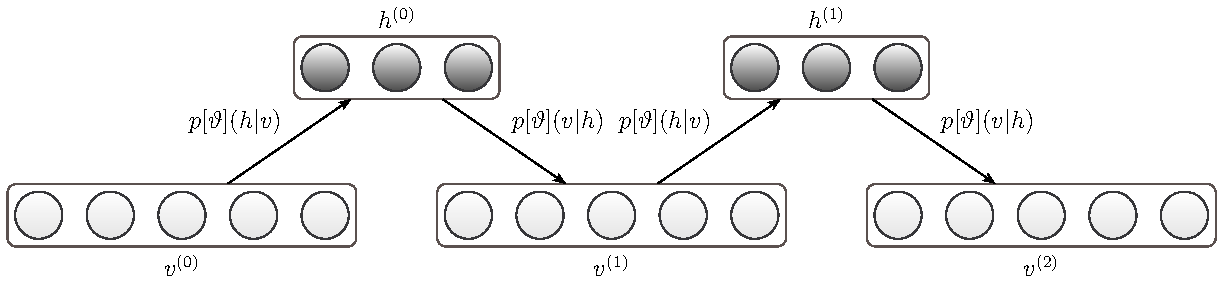
\includegraphics[width=0.9\textwidth]{figures/gibbs-sampling-scheme.pdf}
      \caption{%
        The figure shows the basic scheme of Gibbs sampling.
      }
      \label{fig:gibbs-sampling-scheme}
    \end{figure*}

    The learning procedure for an RBM is rather easy due to its basic structure and good properties.
    First, we need some scalar potential to optimize.
    Learning is always about optimizing some sort of function.
    Because we want to learn a probability distribution on the data set we will use the maximum-likelihood estimation and will try to find a maximum.
    \[
      \mathscr{S} \in V^s
    \]
    As always we will not use the maximum-likelihood function but the log-likelihood function which simplifies the process of computing derivatives and gives us an equivalent optimization condition.
    \[
      \function{\mathscr{L}[\mathscr{S}]}{\setReal^{n\times m + n + m}}{\setReal}
    \]
    \[
      \mathscr{L}[\mathscr{S}](ϑ) \define \frac{1}{s} \sum_{k=1}^s \ln p[ϑ]\roundBrackets{\mathscr{S}_k}
    \]
    We will take one of the simples algorithms to maximize this function.
    \enquote{Gradient Ascent} works exactly like \enquote{Gradient Descent} but finds the maximum instead of the minimum.
    For this we need the gradients of the log-likelihood function with respect to the weight matrix and the bias vectors.
    \[
      \nabla_W \mathscr{L}[\mathscr{S}](ϑ) = \frac{1}{s} \sum_{k=1}^s \expect_ϑ\boxBrackets{\mathscr{V}\transpose{\mathscr{H}} \middle\vert \mathscr{S}_k} - \expect_ϑ\boxBrackets{\mathscr{V}\transpose{\mathscr{H}}}
    \]
    At first sight this formula seems to be complicated.
    But the left part can be easily computed.
    The right part is much more difficult.
    The typical method of finding the expectation of the model itself one has to do Gibbs sampling.
    Figure \ref{fig:gibbs-sampling-scheme} demonstrates this method schematically.

    Using Gibbs sampling for the right part of the gradient is mathematically ideal but fails when applied to reality because the algorithm is slow.
    The typical procedure to make things good again is to abort the series after some given integer.
    Then one can approximate the expectation as follows.
    This is called \enquote{Contrastive Divergence}.
    \[
      \expect_ϑ\boxBrackets{\mathscr{V}\transpose{\mathscr{H}}} \approx v^{(k)}\transpose{h^{(k)}}
    \]
    The algorithm is shown in the following example listing.

    Now one has to talk about the application of the algorithm to collaborative filtering.
    For this every user will get its own RBM which learns only based on the rated and not the unrated movies.
    To not have a set of independent RBMs trained with only one sample one connects the weights and biases of each RBM.
    This means that if two users have rated the same movie then for this movie the same weights and biases will be used.
    Figure \ref{fig:rbm-learning-example} shows the application of this algorithm to the movie ratings by a user again.
    \begin{figure}[H]
      \center
      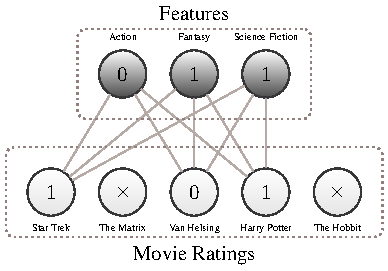
\includegraphics[width=0.441\textwidth]{figures/rbm-learning-example.pdf}
      \caption{%
        The figure shows the application of the learning algorithm to the movie ratings for some user.
      }
      \label{fig:rbm-learning-example}
    \end{figure}
  % section Learning (end)
\end{document}